\documentclass[10pt,a4paper]{article}
\usepackage[utf8]{inputenc}
\usepackage{amsmath}
\usepackage{amssymb}
\usepackage{graphicx}
\usepackage{authblk}
\usepackage{hyperref}
\usepackage{float}
\usepackage{subcaption}

\title{Scattering from Square Conducting Cylinders: A Method of Moments Approach for TE and TM Polarizations}

\author[1]{Yushi Zhou}
\affil[1]{Department of Electrical and Computer Engineering}

\date{\today}

\begin{document}

\maketitle

\begin{abstract}
This paper presents a comprehensive analysis of electromagnetic scattering from infinitely long square conducting cylinders using the Method of Moments (MoM). We investigate both transverse electric (TE) and transverse magnetic (TM) polarizations for normally incident plane waves. The numerical solution implements pulse basis functions and point matching to transform the integral equations into matrix form. We examine cylinders with side lengths of 1$\lambda$ and 3$\lambda$, where $\lambda$ is the wavelength of the incident wave. Results include near-field distributions, bistatic scattering width patterns, and induced surface current densities. The analysis demonstrates how cylinder size affects scattering characteristics and highlights the differences between TE and TM polarizations. 
\end{abstract}

\section{Introduction}
The Method of Moments (MoM) has established itself as one of the most effective numerical techniques for solving electromagnetic scattering problems involving perfect electric conductors (PECs). By transforming integral equations into matrix equations, MoM enables efficient numerical solutions that provide insight into field distributions and scattering patterns.

In this paper, we present a detailed implementation of the MoM for analyzing electromagnetic scattering from infinitely long square conducting cylinders. We consider both transverse electric (TE) and transverse magnetic (TM) polarizations, where the electric or magnetic field, respectively, is parallel to the cylinder axis. The two-dimensional nature of this problem allows us to focus on the cross-sectional electromagnetic behavior.

We investigate cylinders with side lengths of $a = 1\lambda$ and $a = 3\lambda$, where $\lambda$ is the wavelength of the incident plane wave. For each case, we compute and visualize the total field distributions, bistatic scattering widths, and induced surface current densities.

\section{Method}

\subsection{Problem Formulation}

We consider an infinitely long, perfectly conducting square cylinder with side length $a$ located in free space. The cylinder is illuminated by a plane wave propagating in the $-x$ direction. Due to the invariance along the cylinder axis (taken as the $z$-axis), the problem reduces to a two-dimensional analysis in the $xy$-plane.

For TM polarization, the incident electric field is parallel to the cylinder axis:
\begin{equation}
\mathbf{E}^i = E_0 e^{-jk(x\cos\phi_i + y\sin\phi_i)}\hat{z}
\end{equation}

For TE polarization, the incident magnetic field is parallel to the cylinder axis:
\begin{equation}
\mathbf{H}^i = H_0 e^{-jk(x\cos\phi_i + y\sin\phi_i)}\hat{z}
\end{equation}

where $k = 2\pi/\lambda$ is the wavenumber, $\phi_i$ is the incidence angle (taken as $0^\circ$ in our analysis), and $E_0$ and $H_0$ are the amplitudes of the incident fields.

\subsection{Method of Moments Methodology}
The Method of Moments (MoM) is employed to solve the inhomogeneous 2D Helmholtz equation in free space:
\begin{equation}
\nabla^2 \phi(\rho) + k_0^2 \phi(\rho) = f(\rho), \quad \rho \in \Omega_\infty,
\end{equation}
where $\phi(\rho)$ represents the field, $k_0$ is the wavenumber, and $f(\rho)$ is the source term. The corresponding Green's function, which satisfies the inhomogeneous Helmholtz equation, is given by:
\begin{equation}
G_0(\rho, \rho') = \frac{1}{4j} H_0^{(2)}(k_0 |\rho - \rho'|),
\end{equation}
where $H_0^{(2)}$ is the Hankel function of the second kind of order zero. The Green's function also satisfies the Sommerfeld radiation condition:
\begin{equation}
\sqrt{\rho} \left[ \frac{\partial \phi(\rho)}{\partial \rho} + j k_0 \phi(\rho) \right] = 0, \quad \rho \to \infty,
\end{equation}
ensuring that the solution represents outgoing waves at infinity.

When the observation point $\rho$ lies on the boundary $\Gamma_0$ of the scatterer, the field can be expressed using the boundary integral equation\cite{jin2015theory}:
\begin{equation}
\phi^{\text{inc}}(\rho) + \int_{\Gamma_0} \left[ \phi(\rho') \frac{\partial G_0(\rho, \rho')}{\partial n'} - G_0(\rho, \rho') \frac{\partial \phi(\rho')}{\partial n'} \right] \mathrm{d}\Gamma' = \frac{1}{2} \phi(\rho), \quad \rho \in \Gamma_0.
\end{equation}
Here, $\phi^{\text{inc}}(\rho)$ is the incident field, $\phi(\rho')$ is the total field on the boundary, and $\partial / \partial n'$ denotes the derivative normal to the boundary at $\rho'$.

To numerically solve this integral equation, the boundary $\Gamma_0$ is discretized into small segments, and the unknown field $\phi(\rho)$ is approximated using a set of basis functions. The resulting system of equations is then solved to determine the surface currents or equivalent sources, which can be used to compute the scattered fields.

\subsection{Scattering by a Conducting Cylinder}

For TM polarization of an infinitely long square cylinder, the $E_z$ field satisfies:
\begin{equation}
\nabla^2 E_z(\rho) + k_0^2 E_z(\rho) = jk_0 Z_0 J_{i,z}(\rho), \quad \rho \in \Omega_\infty,
\end{equation}
where $k_0$ is the wavenumber, $Z_0$ is the intrinsic impedance of free space, and $J_{i,z}(\rho)$ is the impressed current density.

On the surface of the cylinder, using the equivalence principle, we have:
\begin{equation}
E_z(\rho') = 0, \quad \rho' \in \Gamma_0,
\end{equation}
and
\begin{equation}
\frac{\partial E_z(\rho')}{\partial n'} = jk_0 Z_0 H_t(\rho') = jk_0 Z_0 J_{s,z}(\rho'), \quad \rho' \in \Gamma_0,
\end{equation}
where $J_{s,z}(\rho')$ is the equivalent surface current density.

Substituting these boundary conditions into the integral equation (6), we obtain:
\begin{equation}
E_z^{\text{inc}}(\rho) - jk_0 Z_0 \int_{\Gamma_0} G_0(\rho, \rho') J_{s,z}(\rho') \, \mathrm{d}\Gamma' = 0, \quad \rho \in \Gamma_0,
\end{equation}
which is the Electric Field Integral Equation (EFIE).

To solve this equation numerically, we discretize the surface $\Gamma_0$ into $N$ segments and approximate the surface current $J_{s,z}(\rho')$ using pulse basis functions. This leads to a linear matrix equation:
\begin{equation}
\sum_{n=1}^N Z_{mn} J_{z,n} = V_m, \quad m = 1, 2, \dots, N,
\end{equation}
where
\begin{equation}
Z_{mn} = jk_0 Z_0 \int_{s_n} G_0(\rho_m, \rho') \, \mathrm{d}\Gamma',
\end{equation}
and
\begin{equation}
V_m = E_z^{\text{inc}}(\rho_m).
\end{equation}
Here, $Z_{mn}$ represents the impedance matrix, $J_{z,n}$ is the unknown surface current, and $V_m$ is the excitation vector.

Using the mean value theorem for integrals (we use the midpoint to approximate the integral) and the small argument approximation for the Hankel function, we can derive:
\begin{equation}
Z_{mn} =
\begin{cases}
\frac{k_0 Z_0 s_n}{4} H_0^{(2)}(k_0 |\rho_m - \rho_n|), & m \neq n, \\
\frac{k_0 Z_0 s_n}{4} \left[ 1 - j \frac{2}{\pi} \ln\left(\frac{k_0 \gamma s_n}{4e}\right) \right], & m = n,
\end{cases}
\end{equation}
With the solved surface source $J_{s,z}(\rho')$, we can compute the field at any desired location $\rho \in \Omega_\infty$ using the following expression:

\begin{equation}
E_z(\rho) = E_z^{\text{inc}}(\rho) - jk_0 Z_0 \int_{\Gamma_0} G_0(\rho, \rho') J_{s,z}(\rho') \, \mathrm{d}\Gamma', \quad \rho \in \Omega_\infty.
\end{equation}

For the TE polarization, equations (7), (8), and (9) become:
\begin{equation}
\nabla^2 H_z(\rho) + k_0^2 H_z(\rho) = -[\nabla \times \mathbf{J}_i(\rho)]_z, \quad \rho \in \Omega_\infty,
\end{equation}
and
\begin{equation}
H_z(\rho') = -J_{s,t}(\rho'), \quad \rho' \in \Gamma_0,
\end{equation}
\begin{equation}
\frac{\partial H_z(\rho')}{\partial n'} = 0, \quad \rho' \in \Gamma_0.
\end{equation}

With a similar derivation, we obtain:
\begin{equation}
Z_{mn} = \int_{s_n} \frac{\partial G_0(\rho_m, \rho')}{\partial n'} \, \mathrm{d}\Gamma' - \frac{1}{2} \delta_{mn},
\end{equation}
and
\begin{equation}
V_m = H_z^{\text{inc}}(\rho_m).
\end{equation}
Again, we use midpoint integration and the small argument approximation to get:
\begin{equation}
Z_{mn} =
\begin{cases}
\frac{k_0 s_n}{4j} H_1^{(2)}(k_0 |\rho_m - \rho_n|) \frac{\hat{n}' \cdot (\rho_m - \rho_n)}{|\rho_m - \rho_n|}, & m \neq n, \\
-\frac{1}{2}, & m = n.
\end{cases}
\end{equation}

and then calculate the field at the desired location $\rho \in \Omega_\infty$ using:
\begin{equation}
H_z(\rho) = H_z^{\text{inc}}(\rho) - \int_{\Gamma_0} \frac{\partial G_0(\rho, \rho')}{\partial n'} J_{s,t}(\rho') \, \mathrm{d}\Gamma', \quad \rho \in \Omega_\infty.
\end{equation}









\section{Results and Discussion}

\subsection{Discretization and Convergence study}
The length of square conducting cylinder is set to 1$\lambda$ and 3$\lambda$, respectively. The boundary of the cylinder if discretized into segments of equal length, red nodes in Fig.1(a) shows center of each segment.

\begin{figure}[H]
    \centering
    \begin{subfigure}[b]{0.45\textwidth}
        
\includegraphics[width=\textwidth]{1.jpg}
        \caption{Illustration of discretization.}
    \end{subfigure}
    \hfill
    \begin{subfigure}[b]{0.45\textwidth}
        
\includegraphics[width=\textwidth]{2.jpg}
        \caption{Convergence study of surface current distribution.}
    \end{subfigure}
    \caption{(a) Discretization of the square cylinder boundary into 30 segments each edge. Red nodes indicate the center of each segment. (b) Convergence study for a 1$\lambda$ cylinder with boundary discretized into 10, 20, 30, 50, and 100 segments.}
    \label{fig:discretization_convergence}
\end{figure}

We use the 1$\lambda$ cylinder TM mode to study the convergence of the surface current distribution. The surface current density is calculated for different discretization levels, as shown in Fig.1(b). The results indicate that the surface current density converges as the number of segments increases. The singular point values of the surface current distribution are observed to increase as they approach the theoretical infinite value. However, for a discretization of 30 segments, the results are already accurate enough for practical applications.



\subsection{Surface Current Distribution}
\begin{figure}[H]
    \centering
    \begin{subfigure}[b]{0.45\textwidth}
        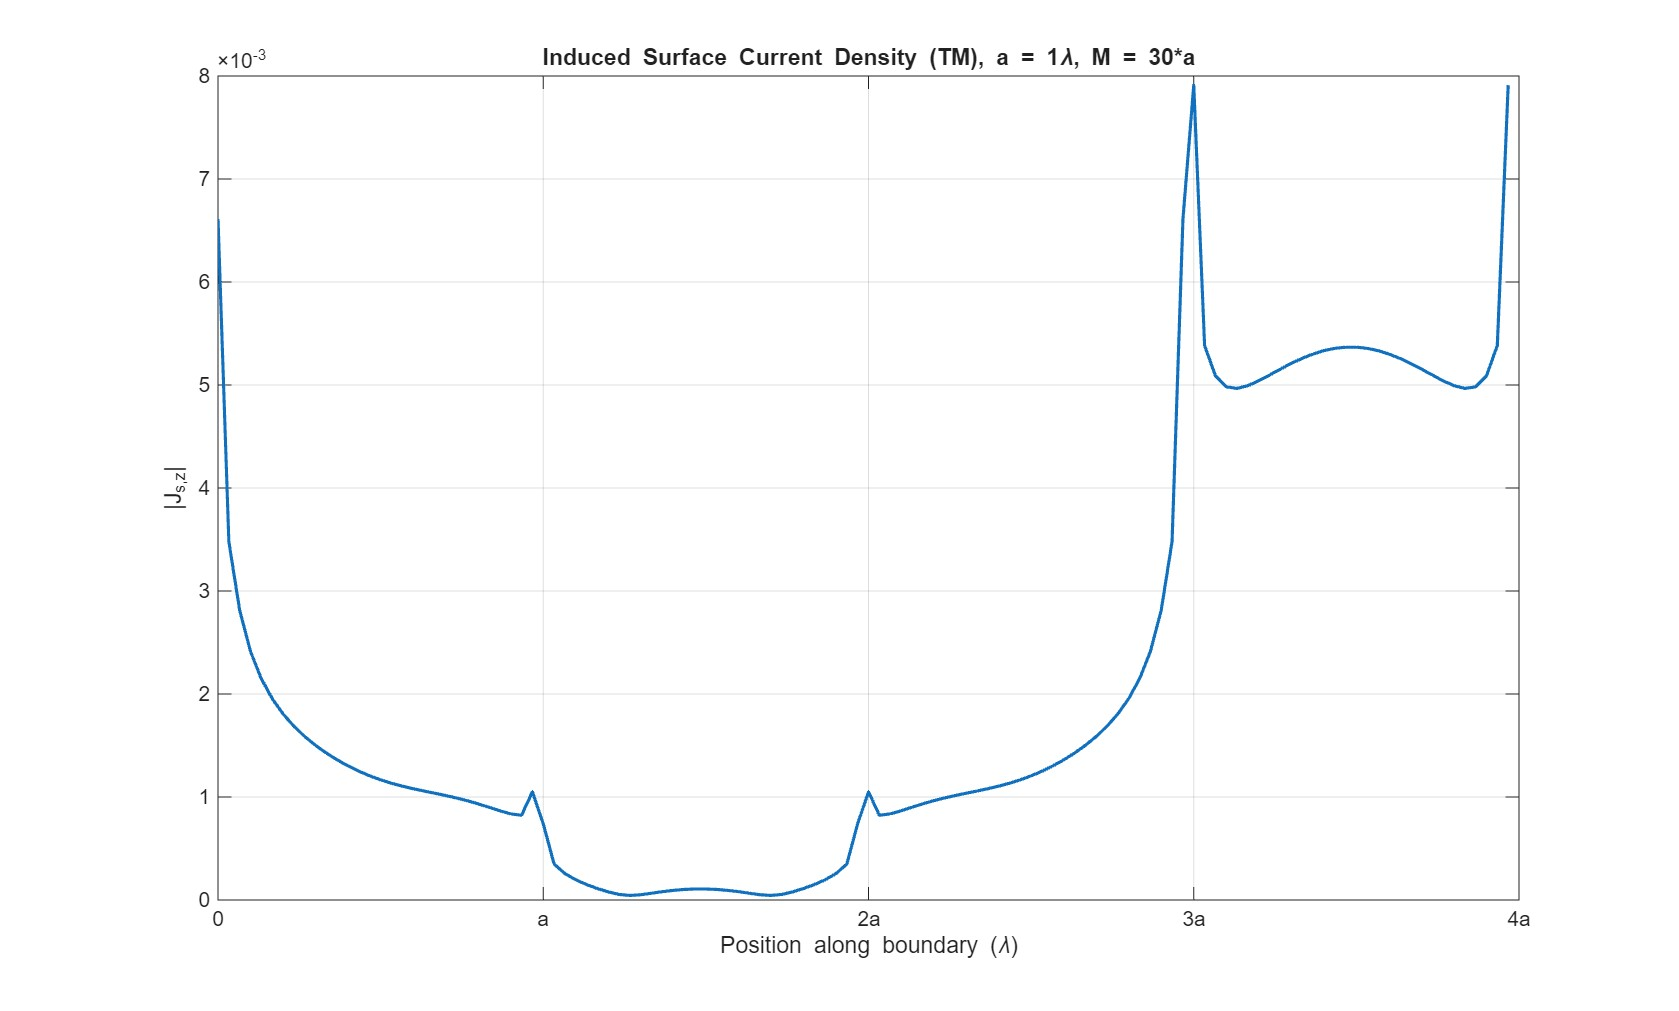
\includegraphics[width=\textwidth]{2a.jpg}
        \caption{TM surface current density $J_{s,z}$ for 1$\lambda$ cylinder.}
    \end{subfigure}
    \hfill
    \begin{subfigure}[b]{0.45\textwidth}
        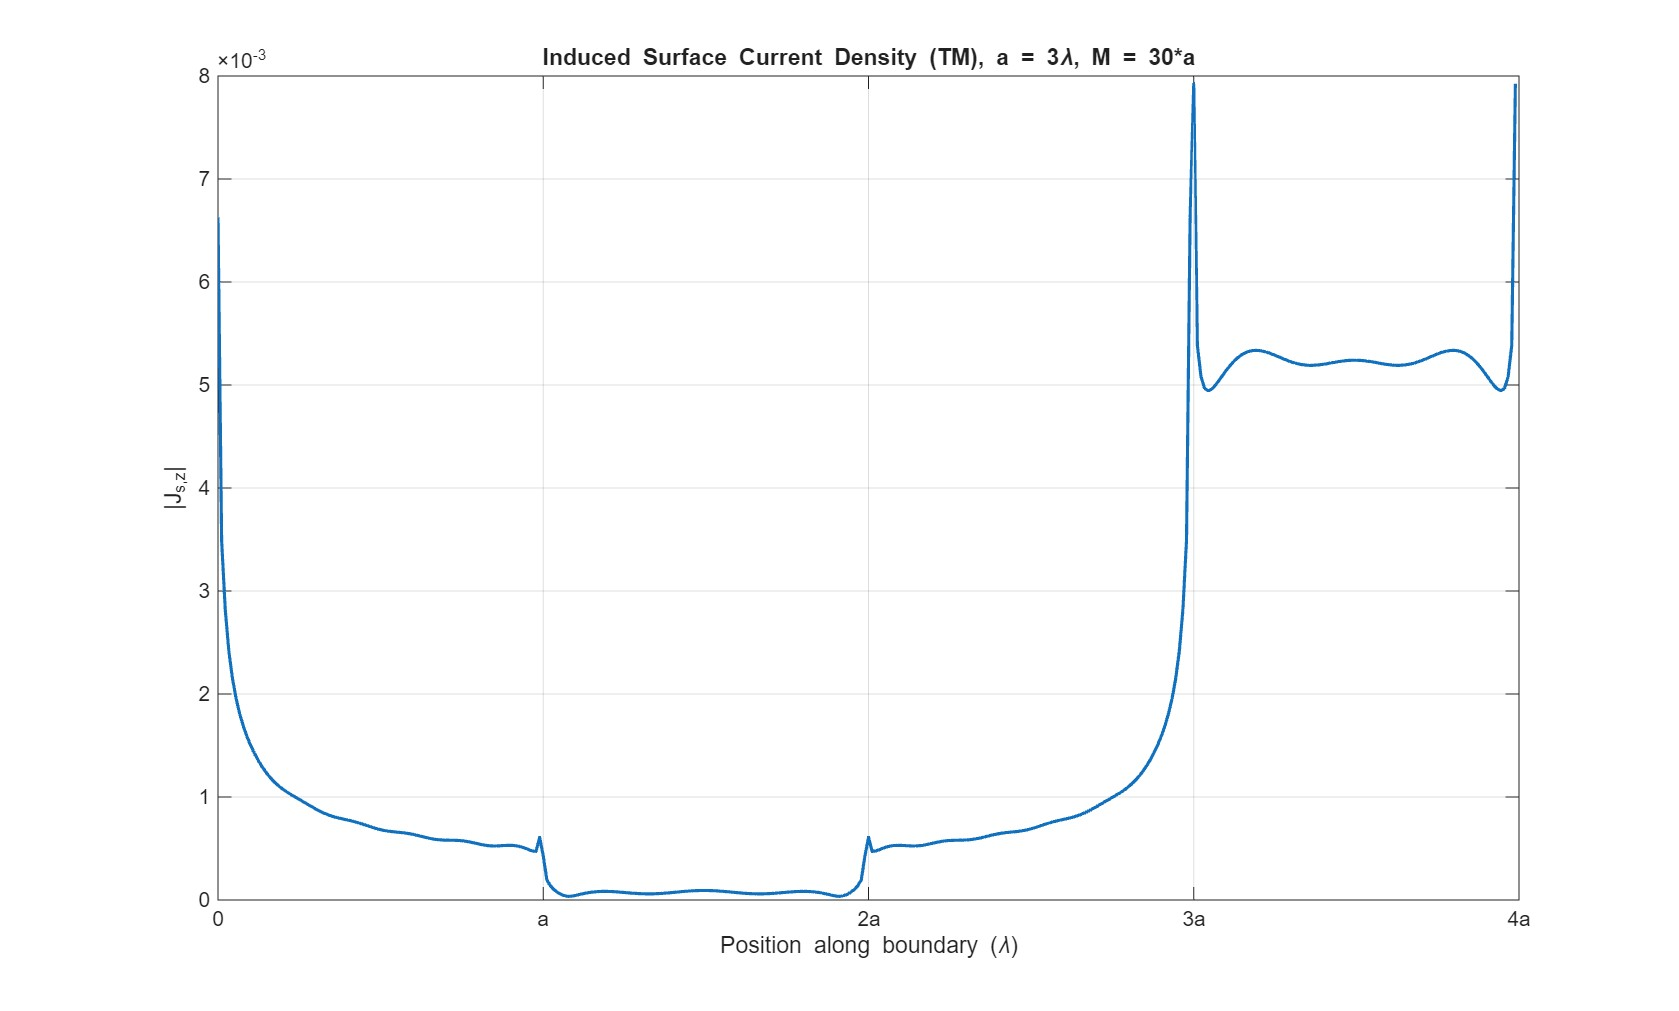
\includegraphics[width=\textwidth]{2b.jpg}
        \caption{TM surface current density $J_{s,z}$ for 3$\lambda$ cylinder.}
    \end{subfigure}
    \hfill
    \begin{subfigure}[b]{0.45\textwidth}
        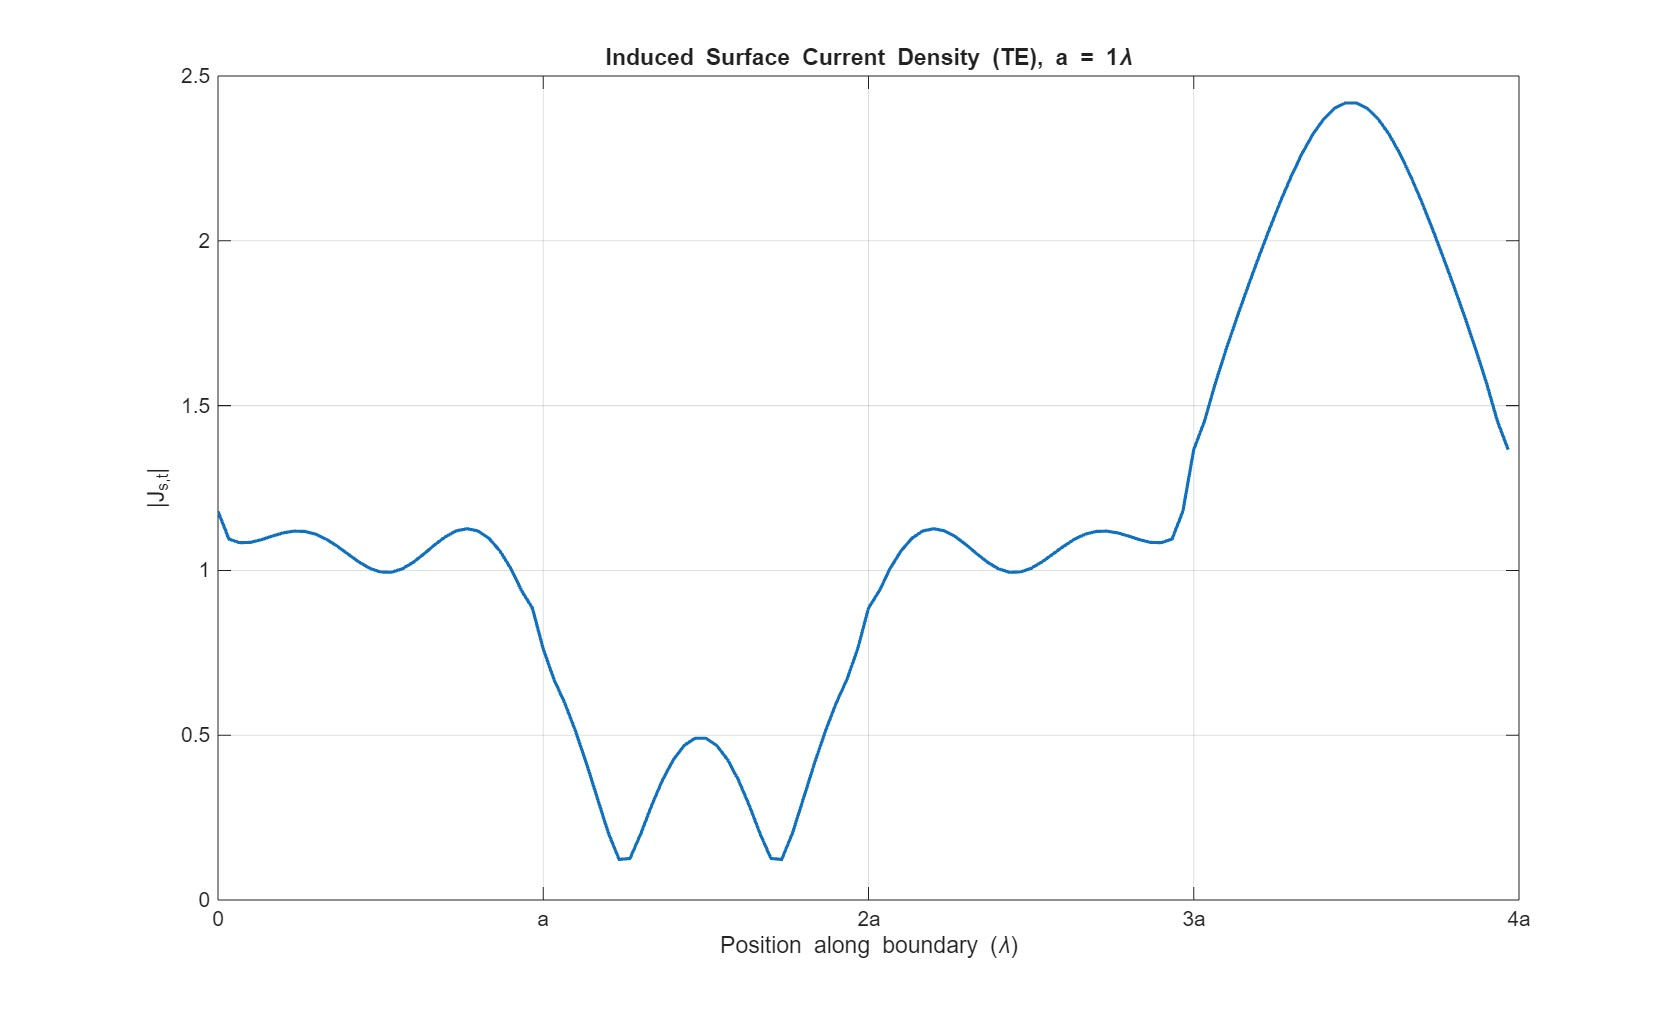
\includegraphics[width=\textwidth]{2c.jpg}
        \caption{TE surface current density $J_{s,t}$ for 1$\lambda$ cylinder.}
    \end{subfigure}
    \hfill
    \begin{subfigure}[b]{0.45\textwidth}
        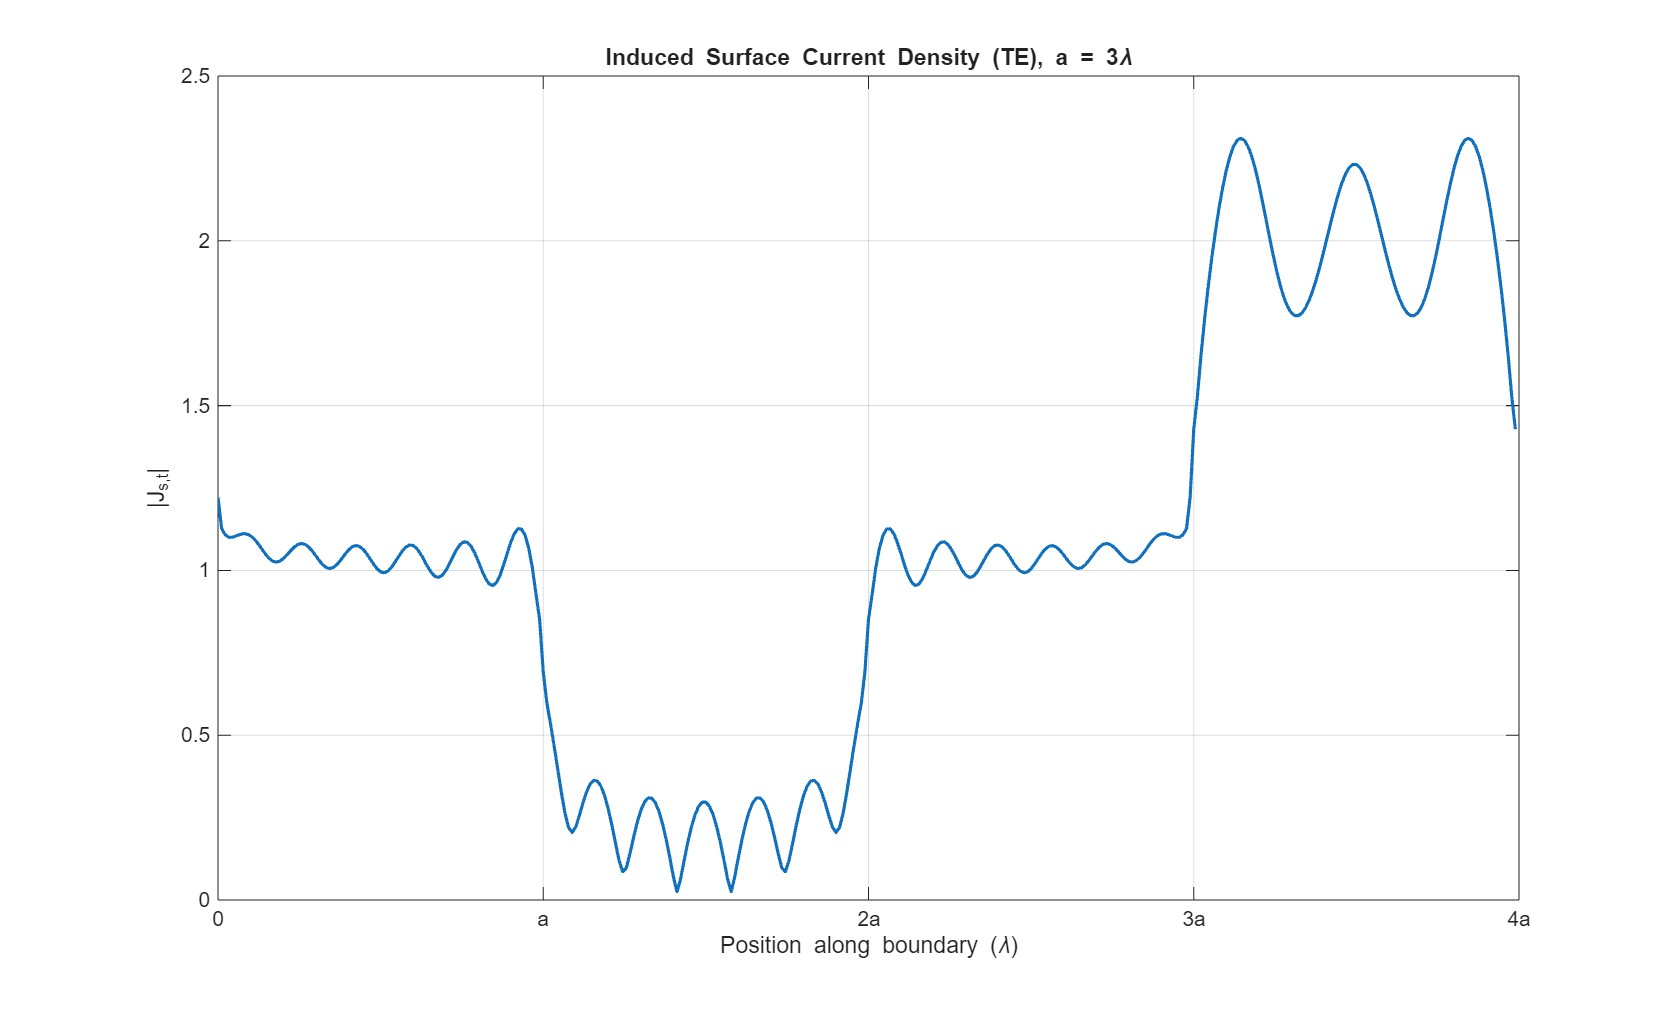
\includegraphics[width=\textwidth]{2d.jpg}
        \caption{TE surface current density $J_{s,t}$ for 3$\lambda$ cylinder.}
    \end{subfigure}
    \caption{Surface current distributions for TM and TE polarizations. (a) and (b) show the TM surface current density $J_{s,z}$ for 1$\lambda$ and 3$\lambda$ cylinders, respectively. (c) and (d) show the TE surface current density $J_{s,t}$ for 1$\lambda$ and 3$\lambda$ cylinders, respectively.}
    \label{fig:surface_current}
\end{figure}

For TM polarization, the surface current density $J_{s,z}$ exhibits sharp peaks at the corners due to charge accumulation caused by the discontinuity in the tangential electric field. 

In contrast, for TE polarization, the surface current density $J_{s,t}$ remains continuous at the corners because the magnetic field boundary conditions do not induce charge accumulation. Instead, the TE case shows surface standing waves along the cylinder boundary, arising from constructive and destructive interference of counter-propagating surface waves. These waves are absent in the TM case due to the lack of tangential electric field components on the surface.


\subsection{Field Distributions}
\begin{figure}[H]
    \centering
    \begin{subfigure}[b]{0.4\textwidth}
        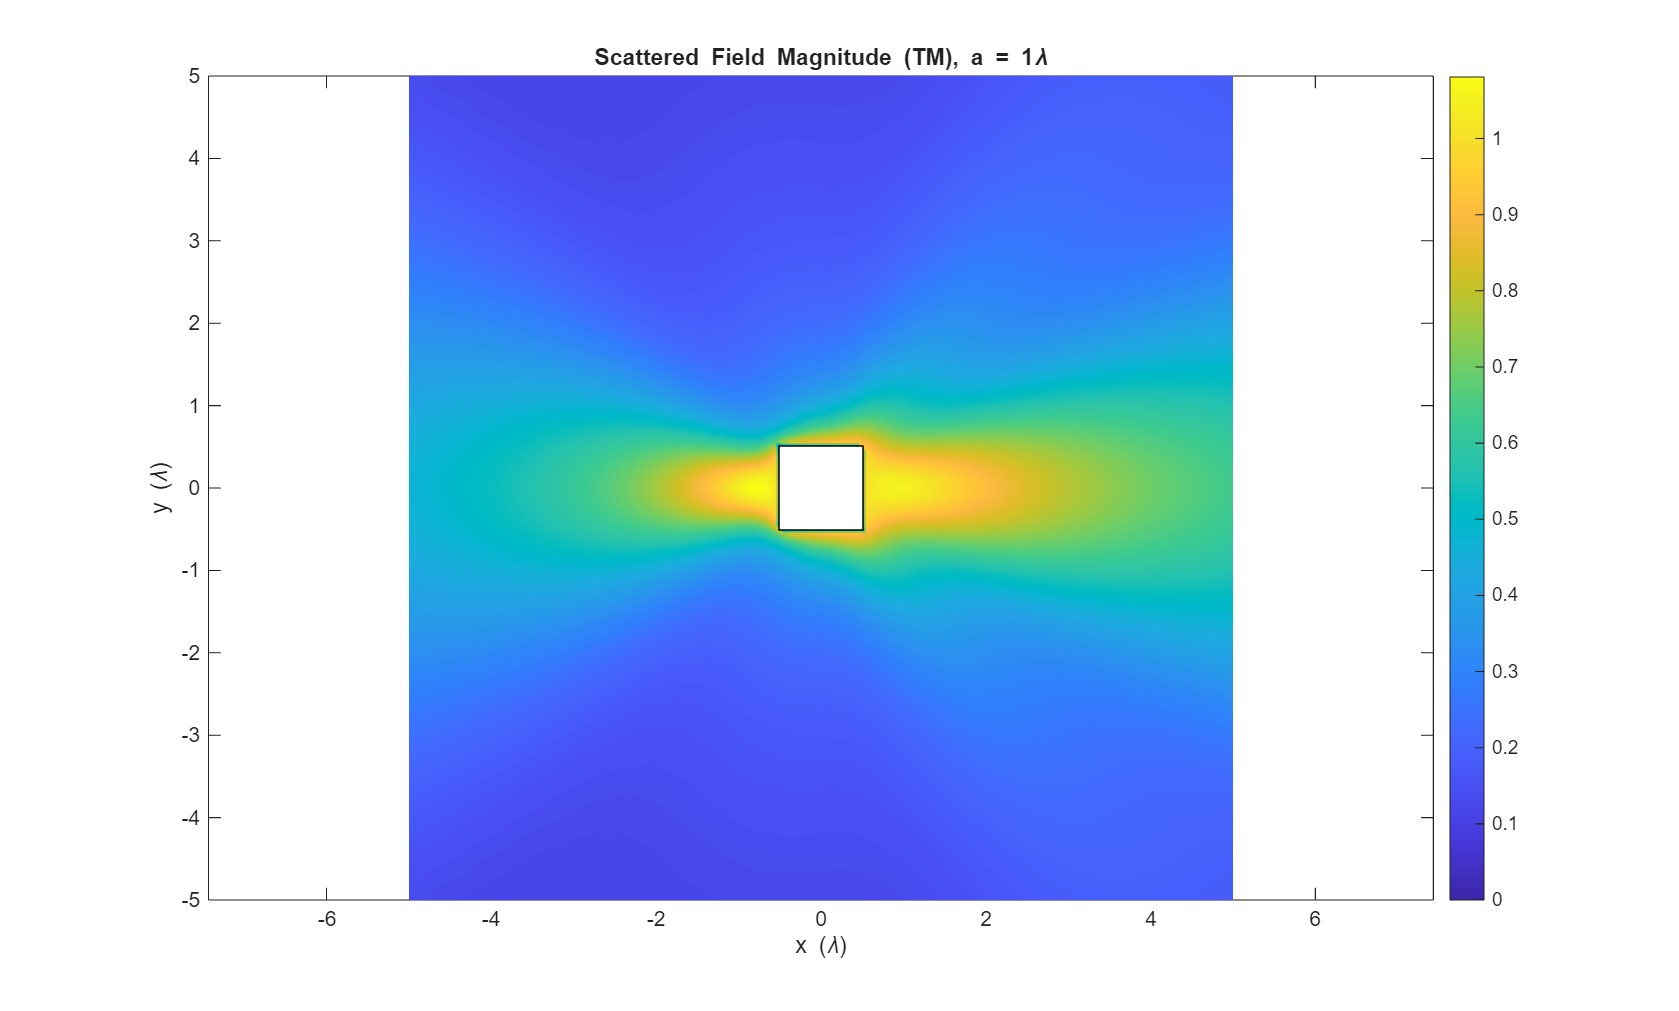
\includegraphics[width=\textwidth]{3a.jpg}
        \caption{Scattered field for TM polarization, 1$\lambda$ cylinder.}
    \end{subfigure}
    \hfill
    \begin{subfigure}[b]{0.4\textwidth}
        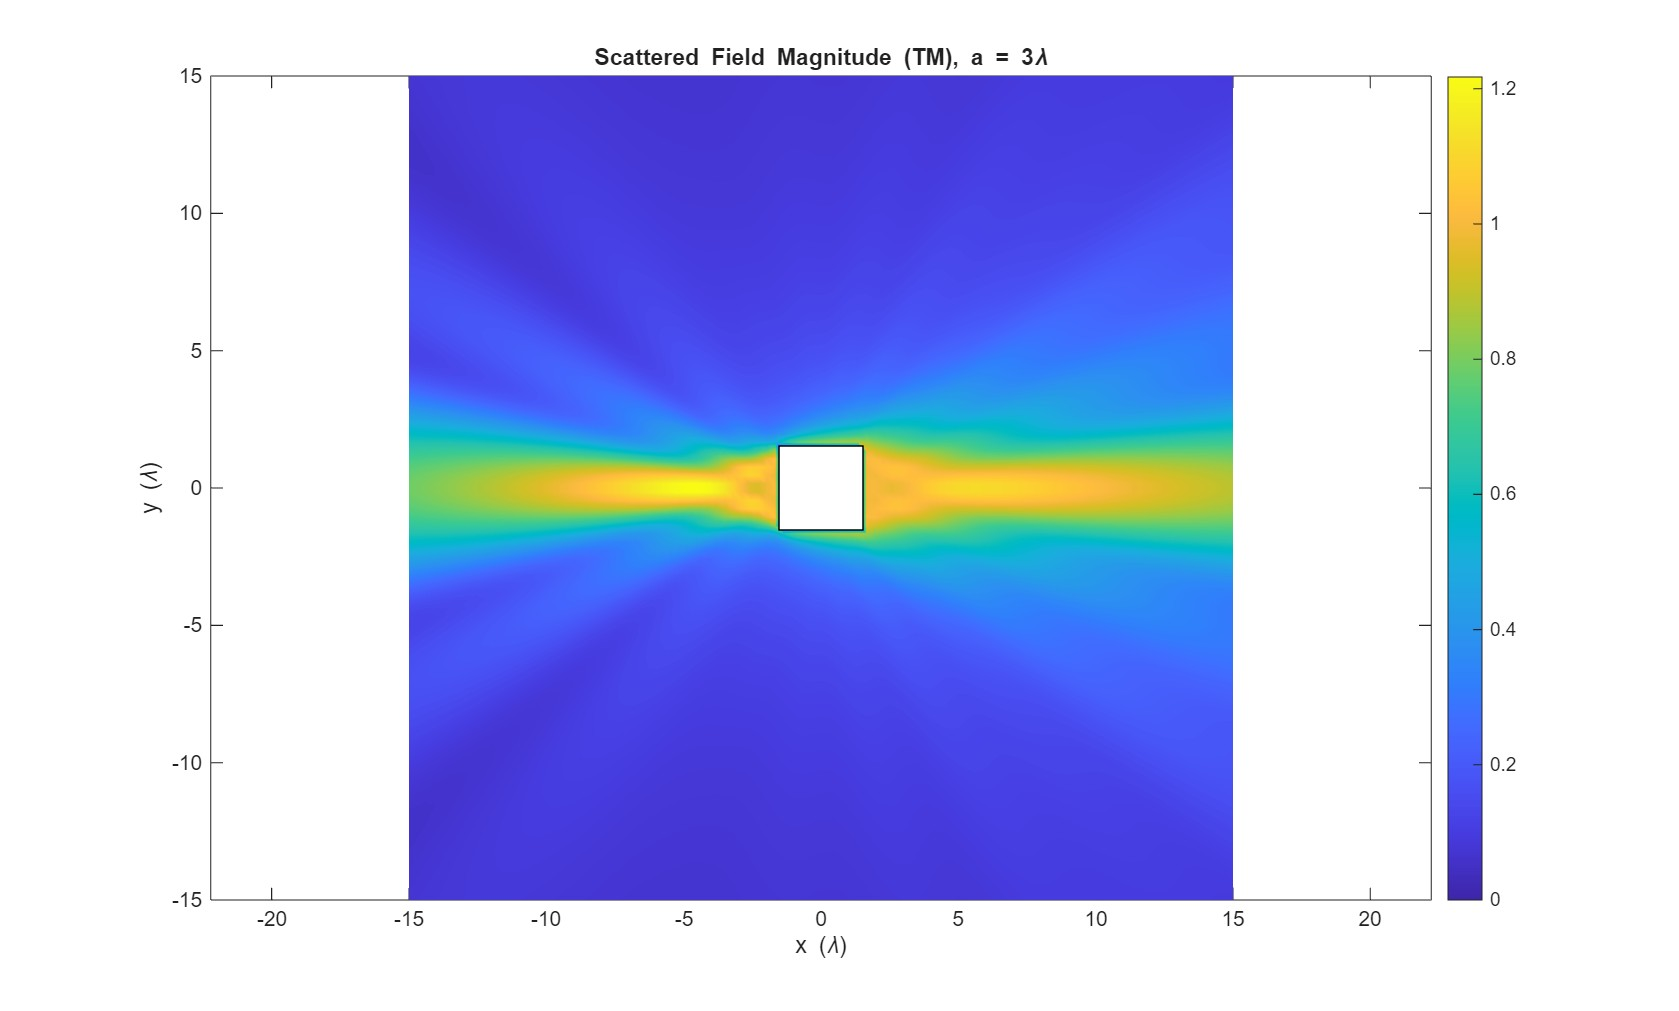
\includegraphics[width=\textwidth]{3b.jpg}
        \caption{Scattered field for TM polarization, 3$\lambda$ cylinder.}
    \end{subfigure}
    \hfill
    \begin{subfigure}[b]{0.4\textwidth}
        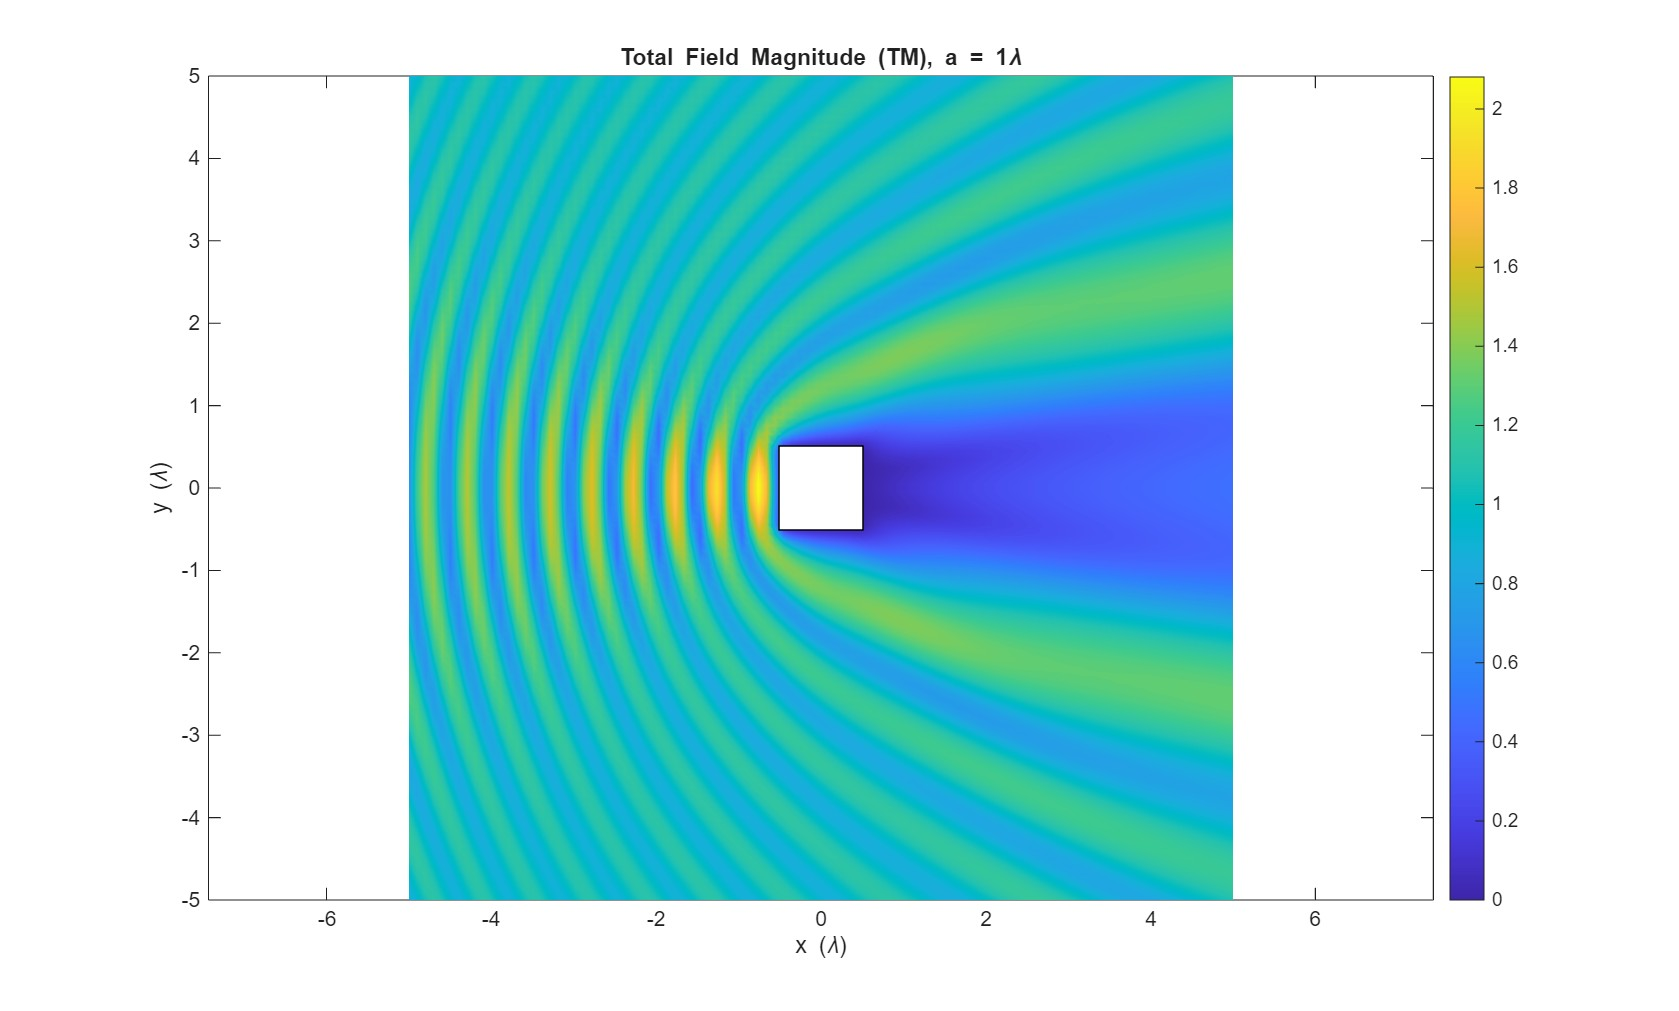
\includegraphics[width=\textwidth]{3c.jpg}
        \caption{Total field for TM polarization, 1$\lambda$ cylinder.}
    \end{subfigure}
    \hfill
    \begin{subfigure}[b]{0.4\textwidth}
        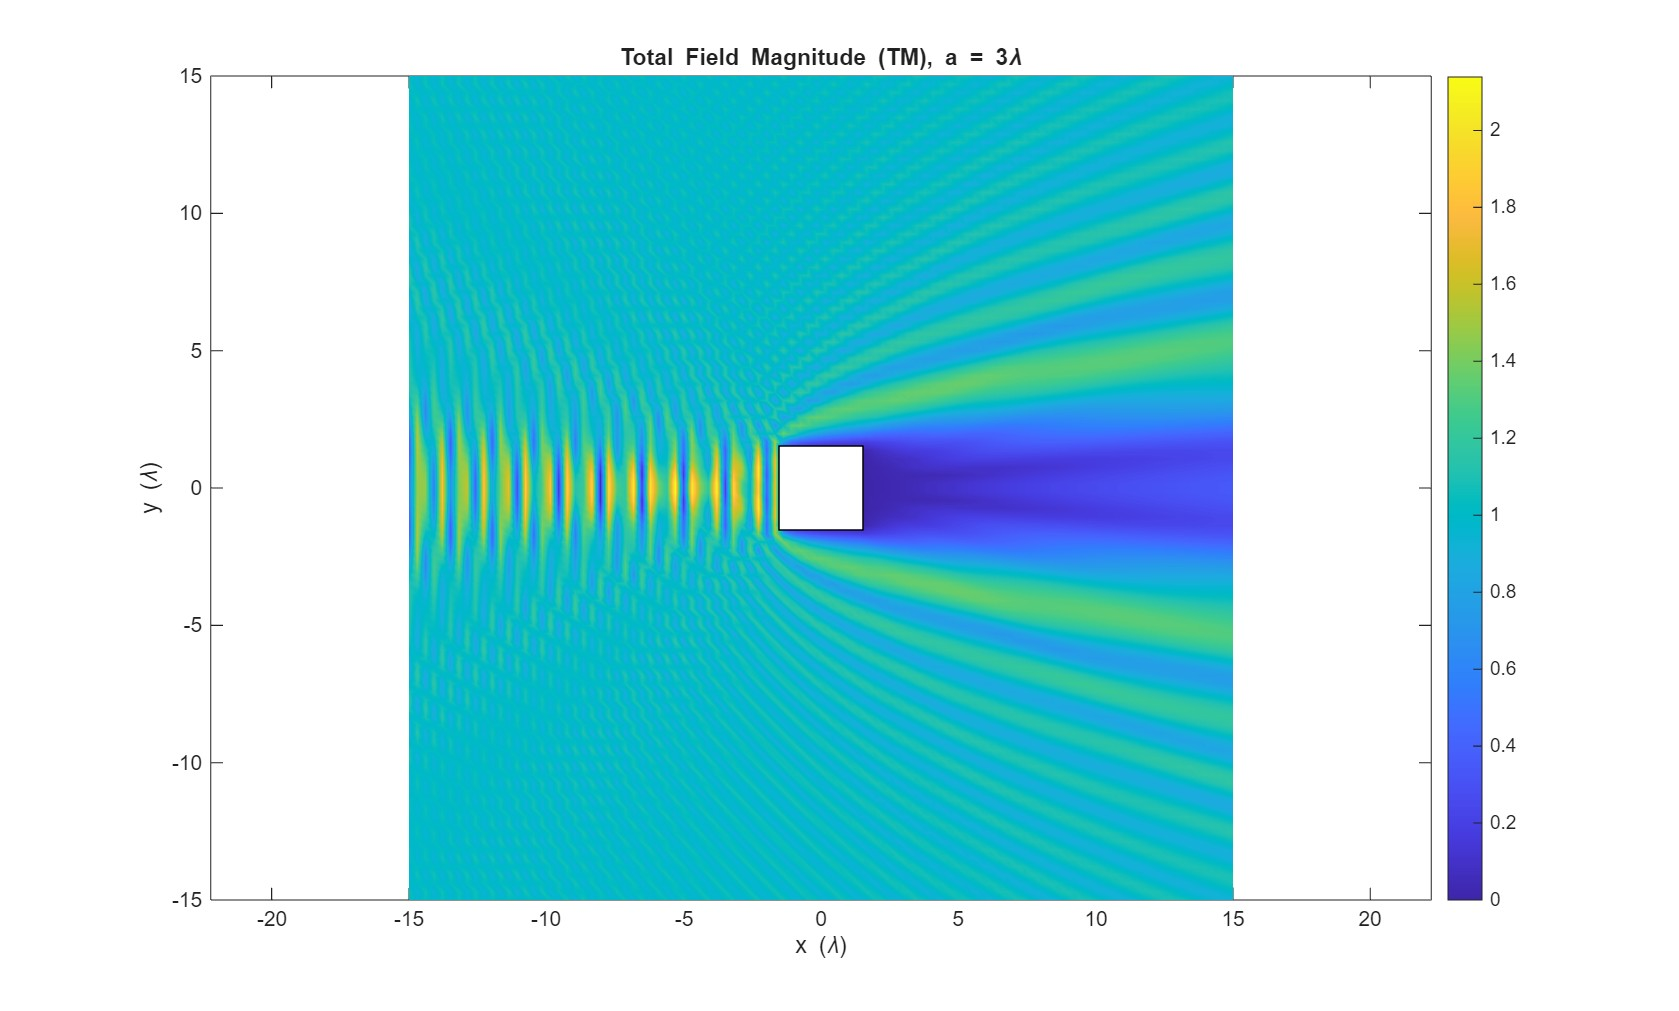
\includegraphics[width=\textwidth]{3d.jpg}
        \caption{Total field for TM polarization, 3$\lambda$ cylinder.}
    \end{subfigure}
    \caption{Field distributions for TM polarization. (a) and (b) show the scattered field for 1$\lambda$ and 3$\lambda$ cylinders, respectively. (c) and (d) show the total field for 1$\lambda$ and 3$\lambda$ cylinders, respectively.}
    \label{fig:field_distributions}
\end{figure}
\begin{figure}[H]
    \centering
    \begin{subfigure}[b]{0.4\textwidth}
        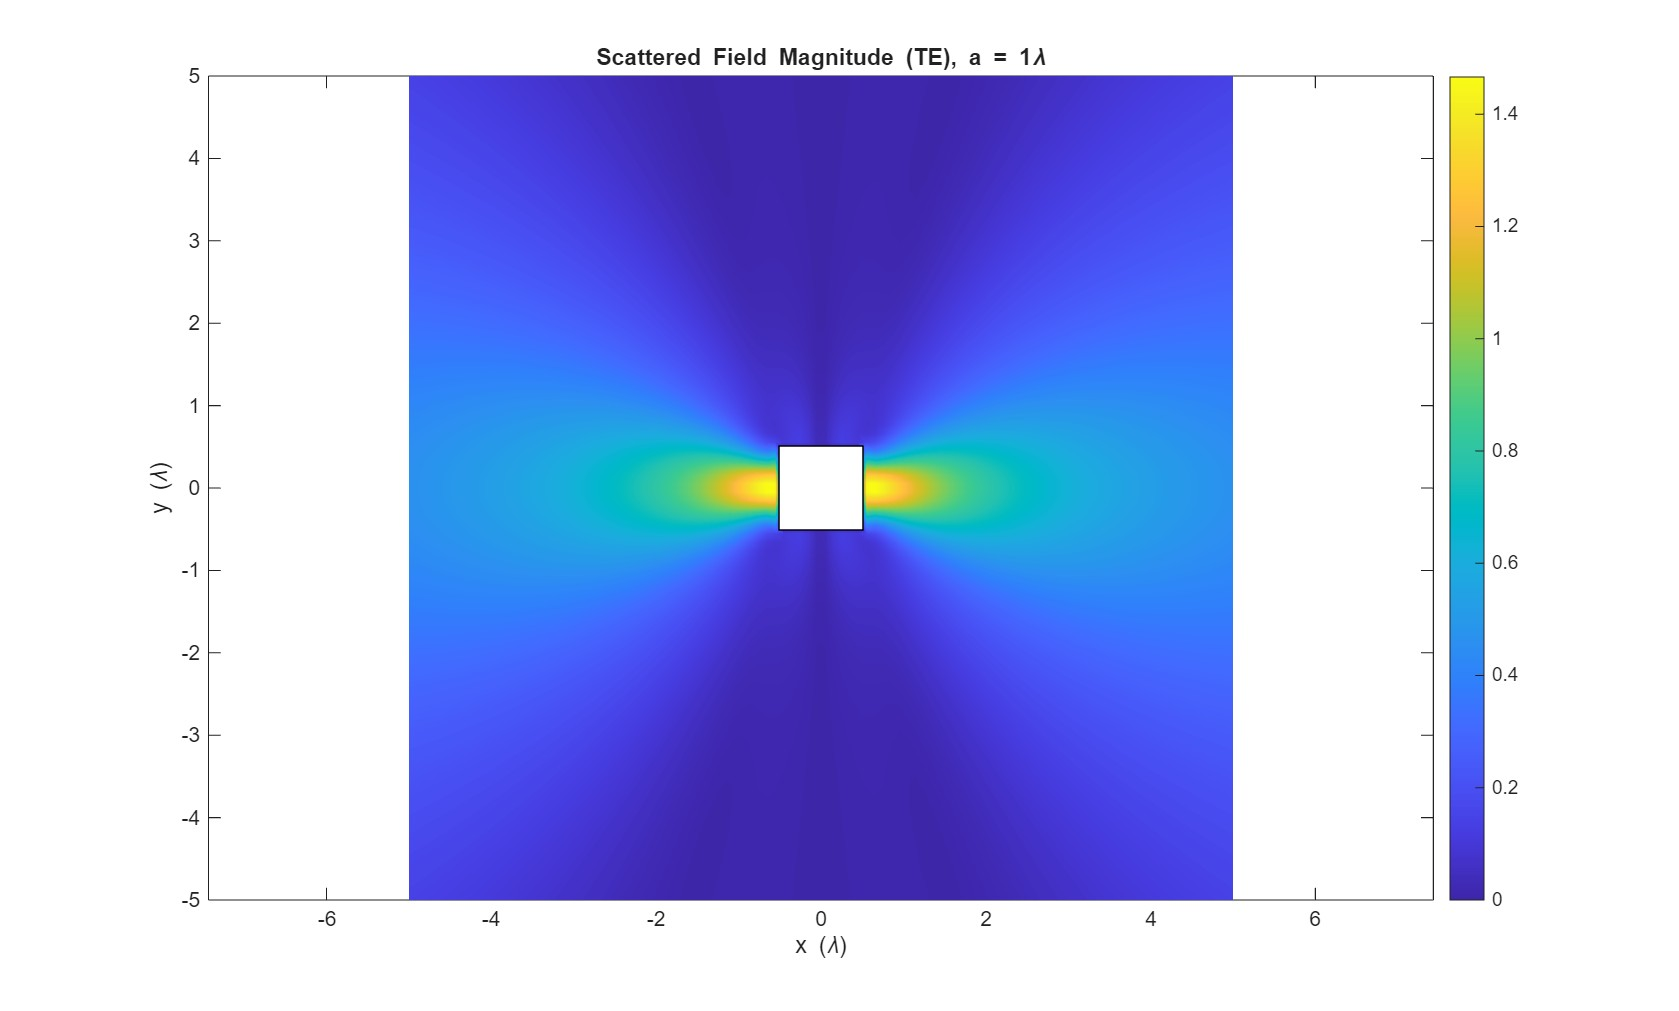
\includegraphics[width=\textwidth]{4a.jpg}
        \caption{Scattered field for TE polarization, 1$\lambda$ cylinder.}
    \end{subfigure}
    \hfill
    \begin{subfigure}[b]{0.4\textwidth}
        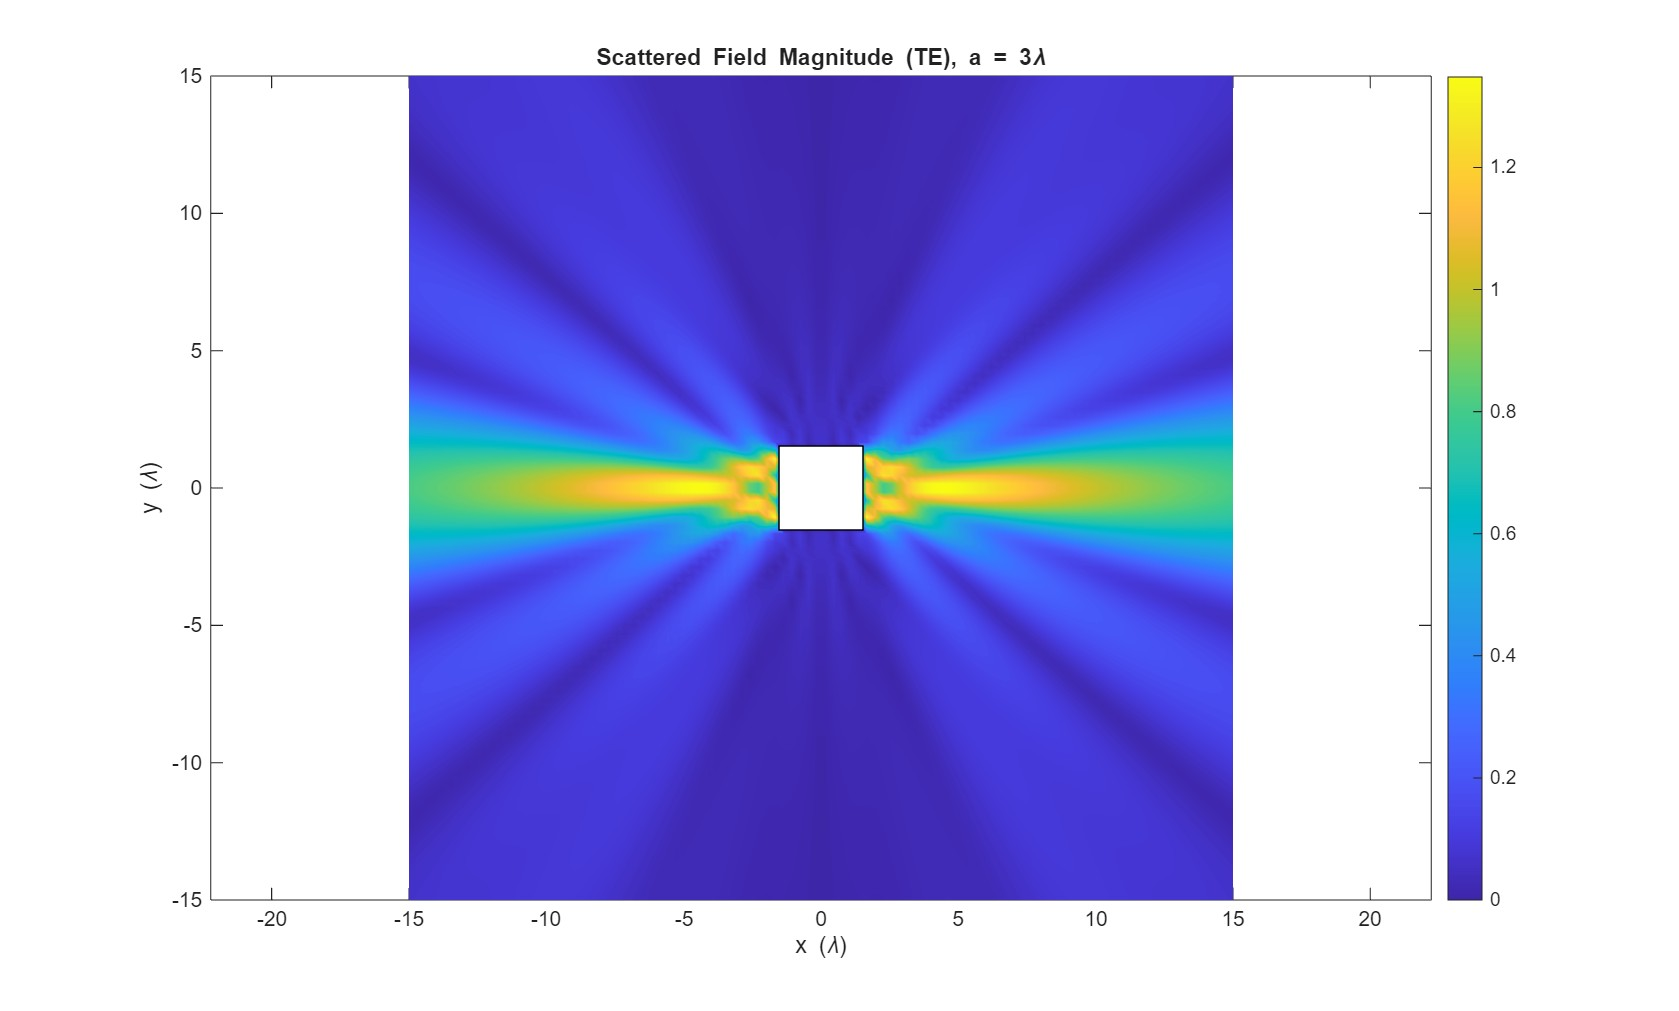
\includegraphics[width=\textwidth]{4b.jpg}
        \caption{Scattered field for TE polarization, 3$\lambda$ cylinder.}
    \end{subfigure}
    \hfill
    \begin{subfigure}[b]{0.4\textwidth}
        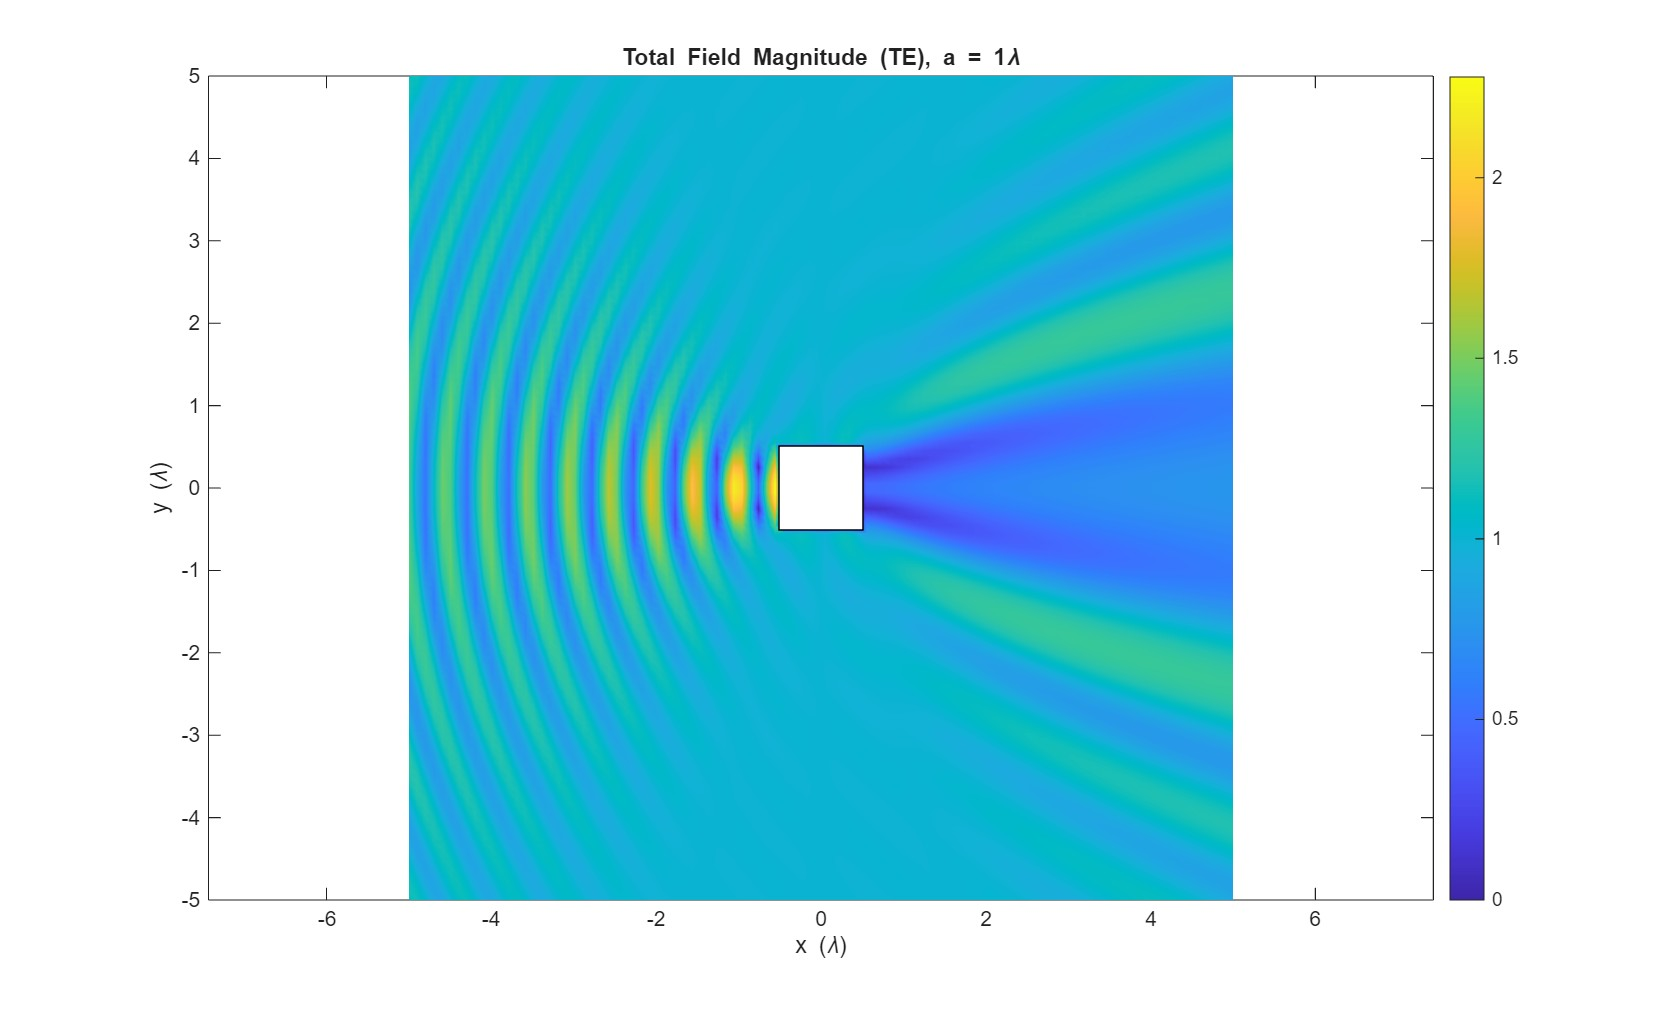
\includegraphics[width=\textwidth]{4c.jpg}
        \caption{Total field for TE polarization, 1$\lambda$ cylinder.}
    \end{subfigure}
    \hfill
    \begin{subfigure}[b]{0.4\textwidth}
        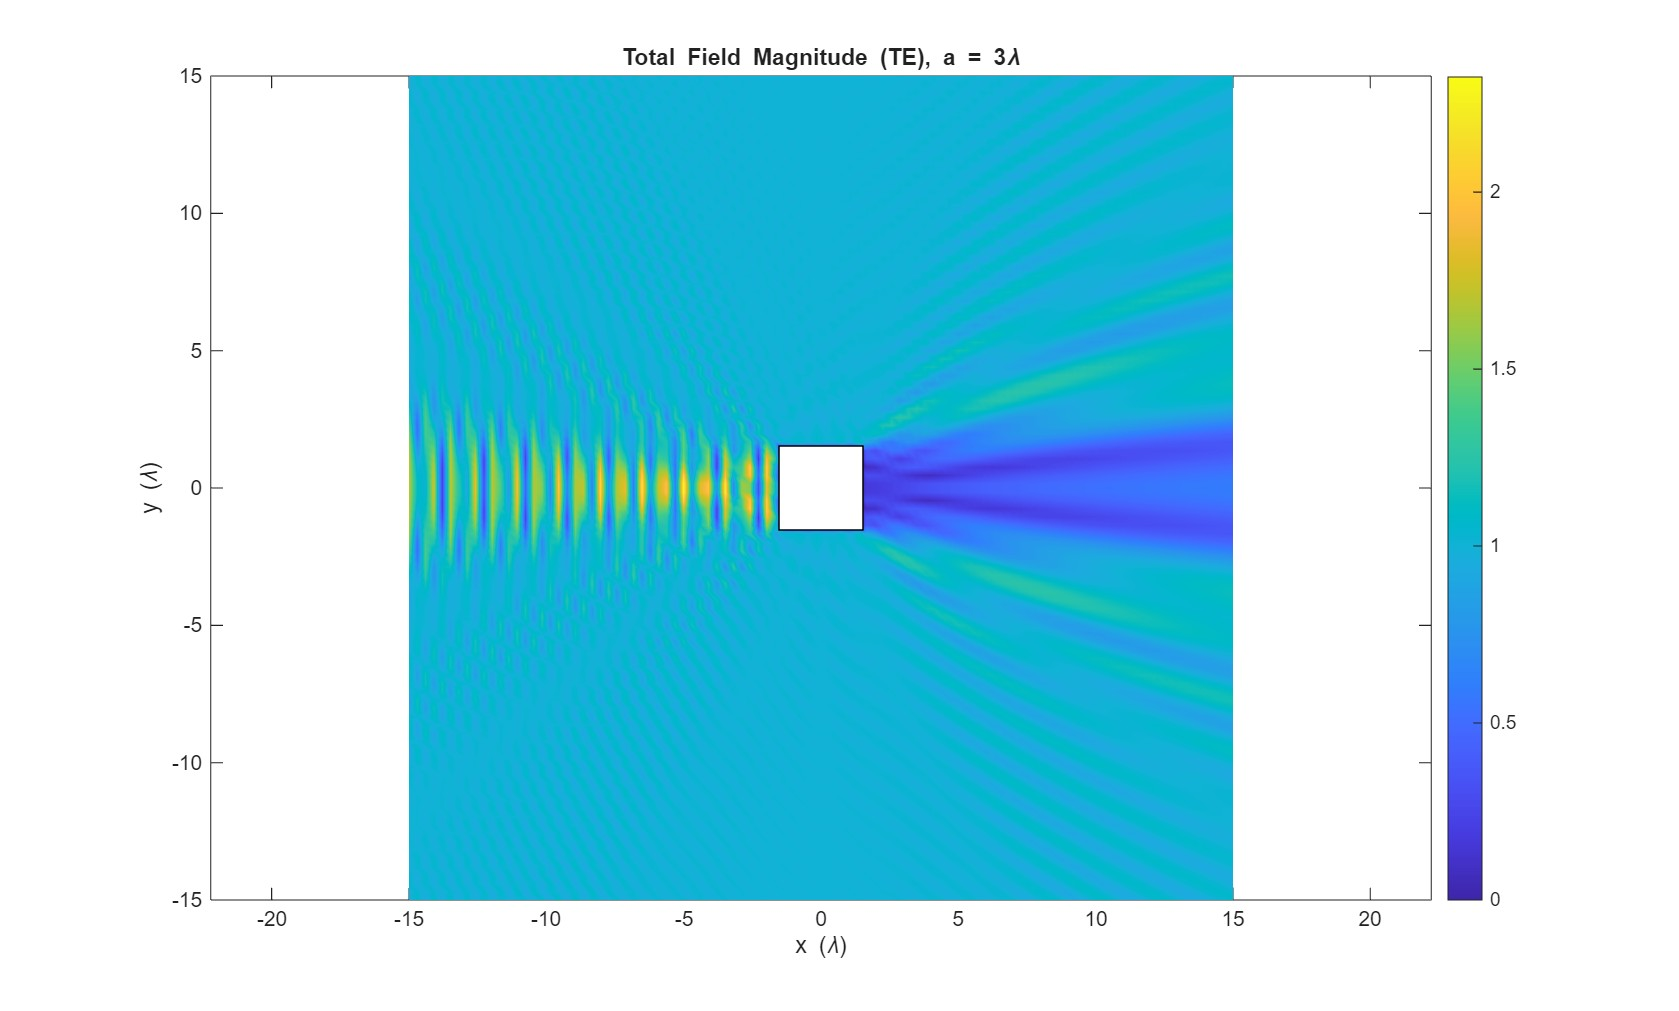
\includegraphics[width=\textwidth]{4d.jpg}
        \caption{Total field for TE polarization, 3$\lambda$ cylinder.}
    \end{subfigure}
    \caption{Field distributions for TE polarization. (a) and (b) show the scattered field for 1$\lambda$ and 3$\lambda$ cylinders, respectively. (c) and (d) show the total field for 1$\lambda$ and 3$\lambda$ cylinders, respectively.}
    \label{fig:field_distributions_te}
\end{figure}

Fig.3 and Fig.4 illustrate the scattered and total field distributions for TM and TE polarizations, respectively. The interference patterns observed in the total field distributions result from the superposition of the incident and scattered fields. For the 1$\lambda$ cylinder, the interference pattern is relatively simple, with clear constructive and destructive regions. In contrast, for the 3$\lambda$ cylinder, the patterns become more complex due to the larger electrical size, leading to multiple lobes and higher-order interactions.
\subsection{Bistatic Scattering Width}

The bistatic scattering width, which characterizes the angular distribution of scattered power, is calculated for scattering angles ranging from 0° to 360°.

\begin{figure}[H]
    \centering
    \begin{subfigure}[b]{0.45\textwidth}
        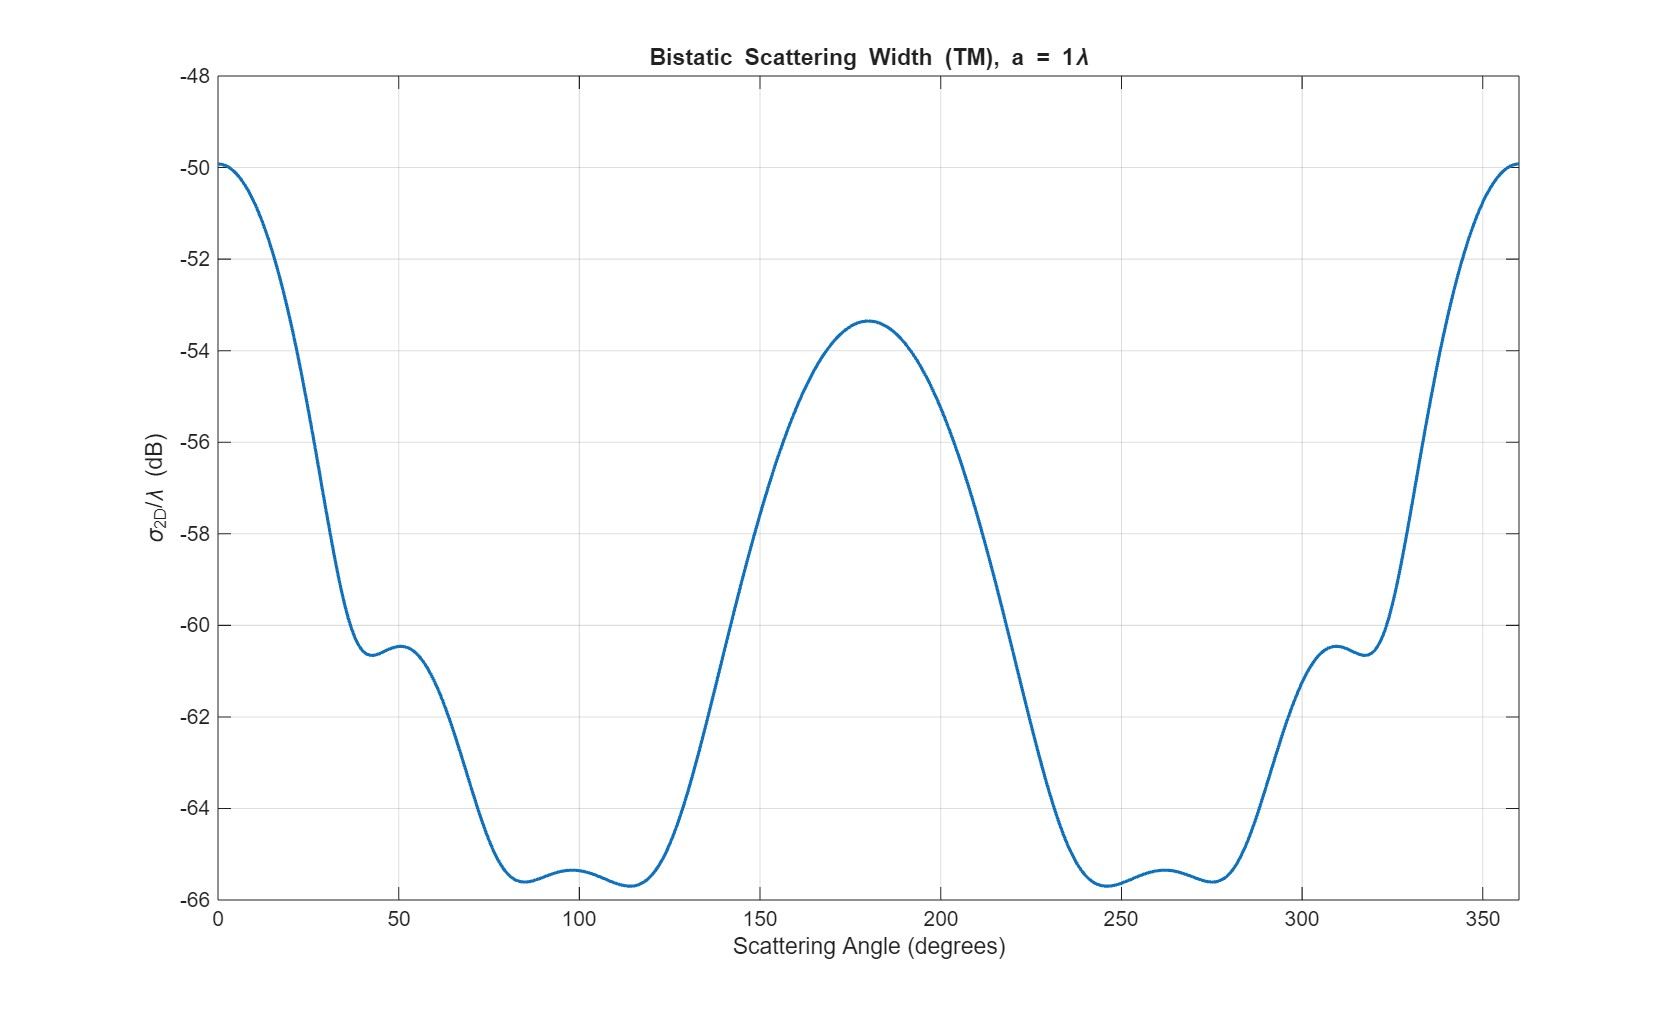
\includegraphics[width=\textwidth]{5a.jpg}
        \caption{TM bistatic scattering width for 1$\lambda$ cylinder.}
    \end{subfigure}
    \hfill
    \begin{subfigure}[b]{0.45\textwidth}
        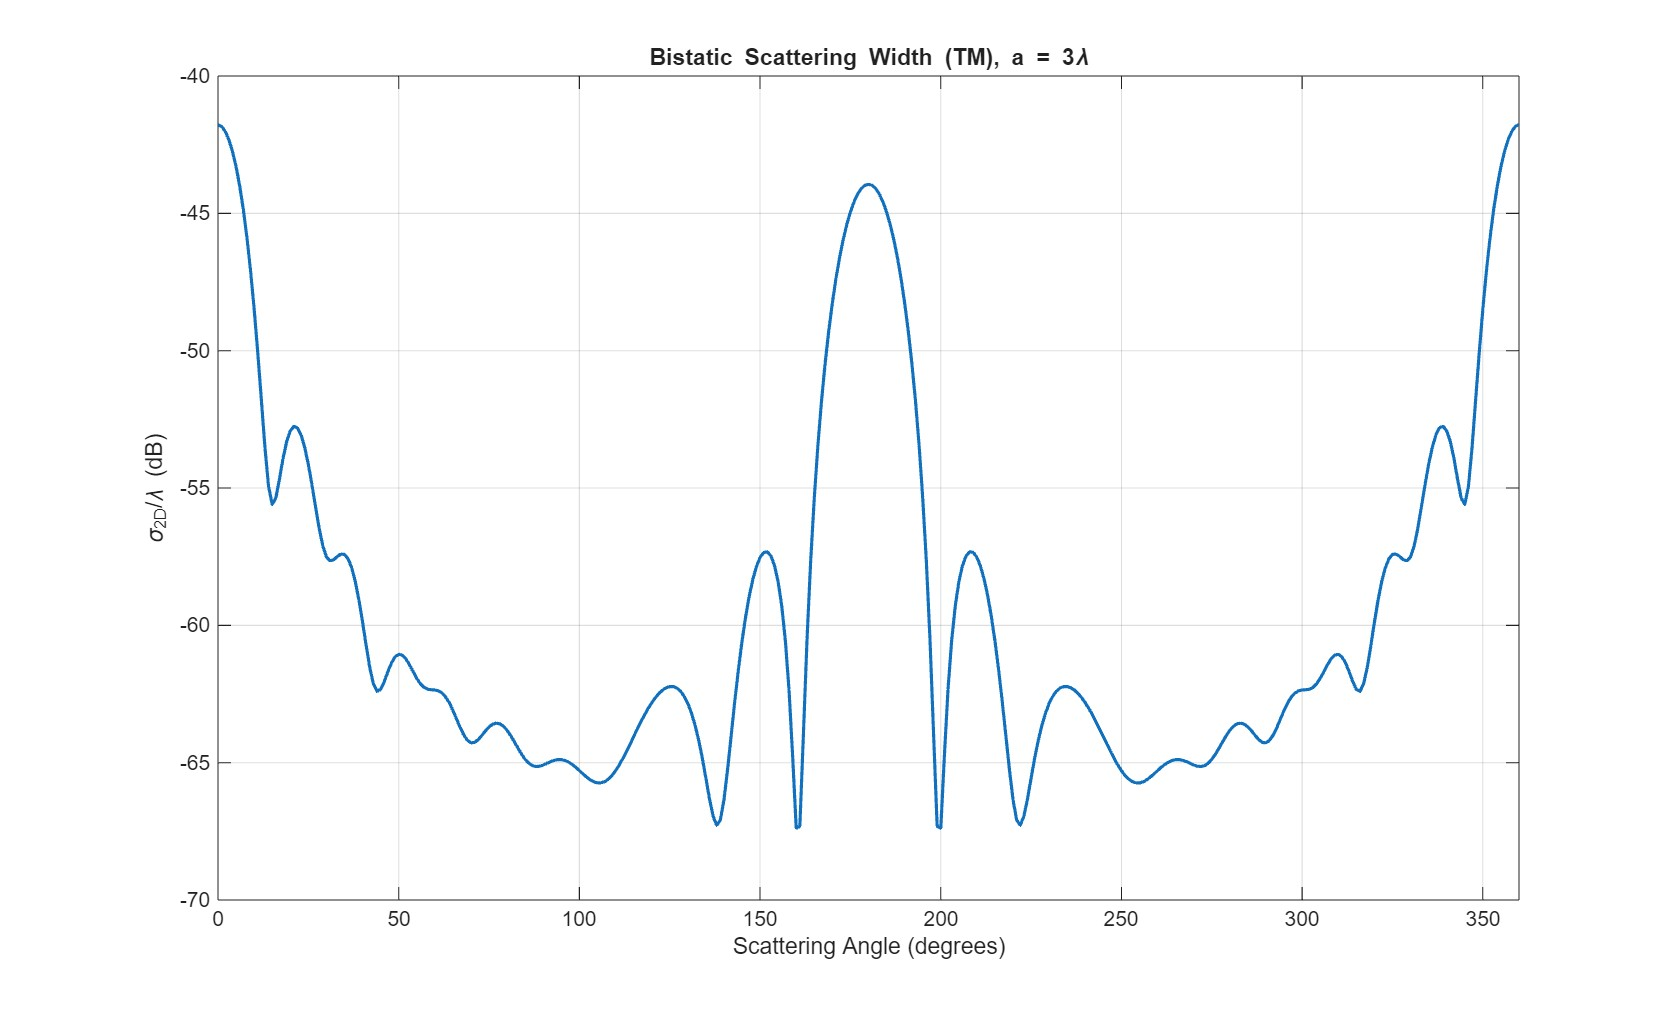
\includegraphics[width=\textwidth]{5b.jpg}
        \caption{TM bistatic scattering width for 3$\lambda$ cylinder.}
    \end{subfigure}
    \hfill
    \begin{subfigure}[b]{0.45\textwidth}
        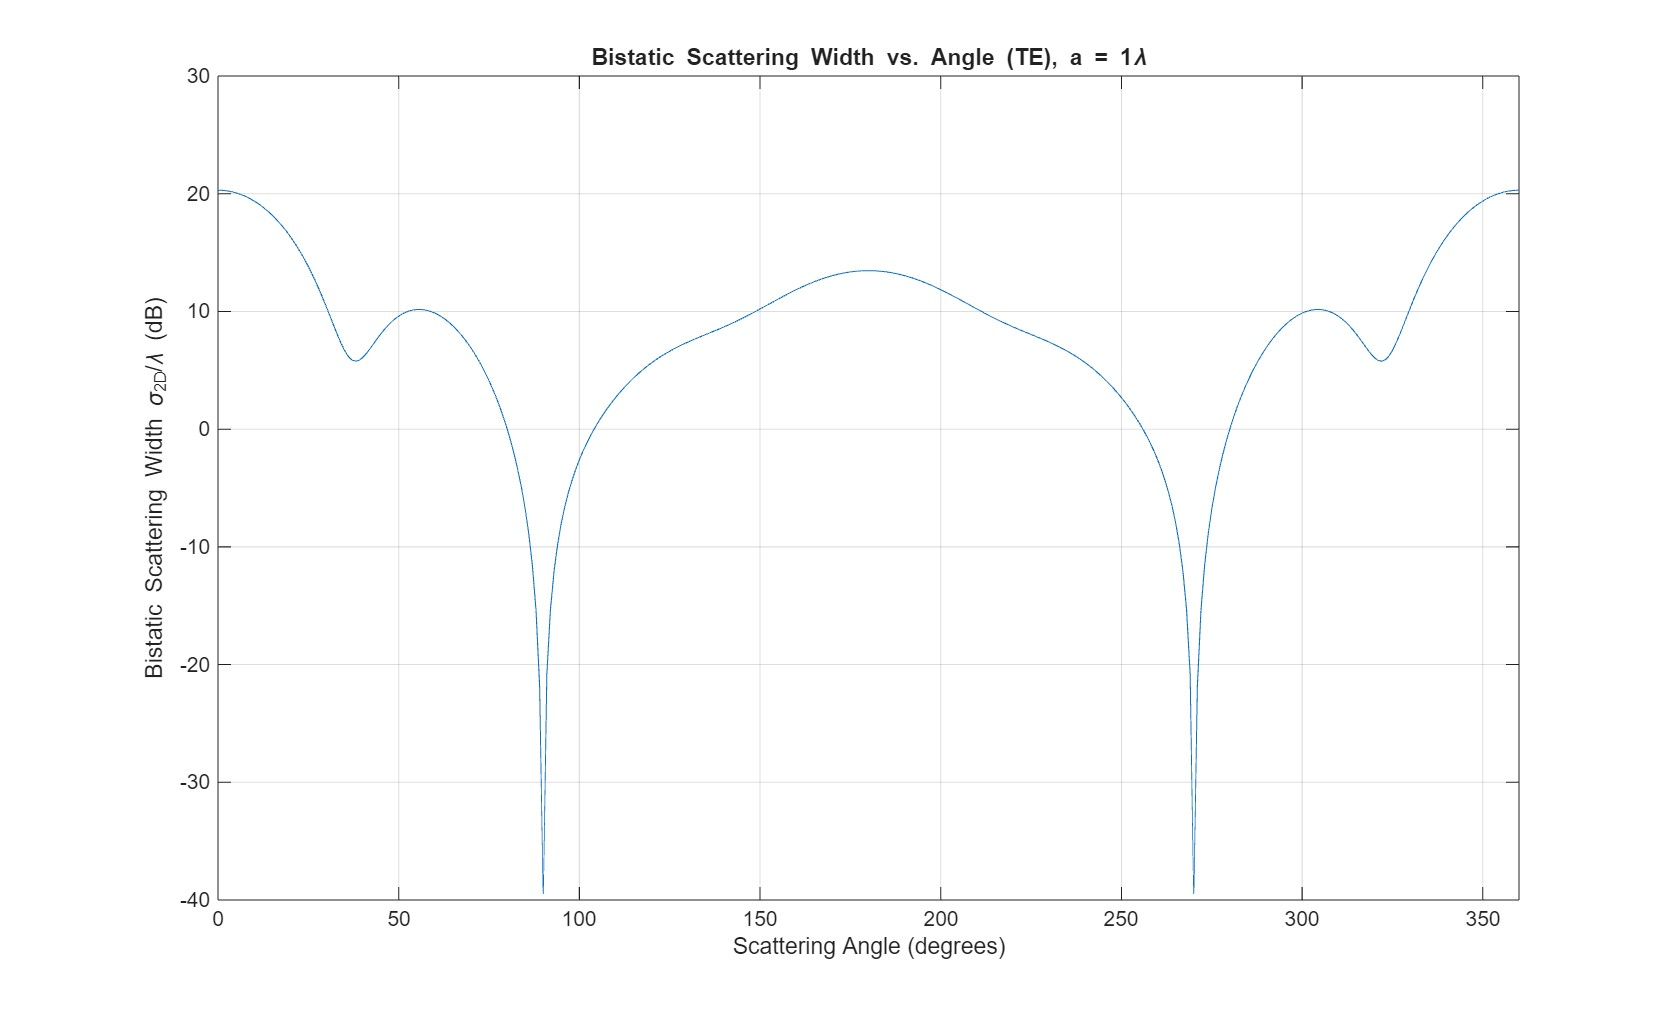
\includegraphics[width=\textwidth]{5c.jpg}
        \caption{TE bistatic scattering width for 1$\lambda$ cylinder.}
    \end{subfigure}
    \hfill
    \begin{subfigure}[b]{0.45\textwidth}
        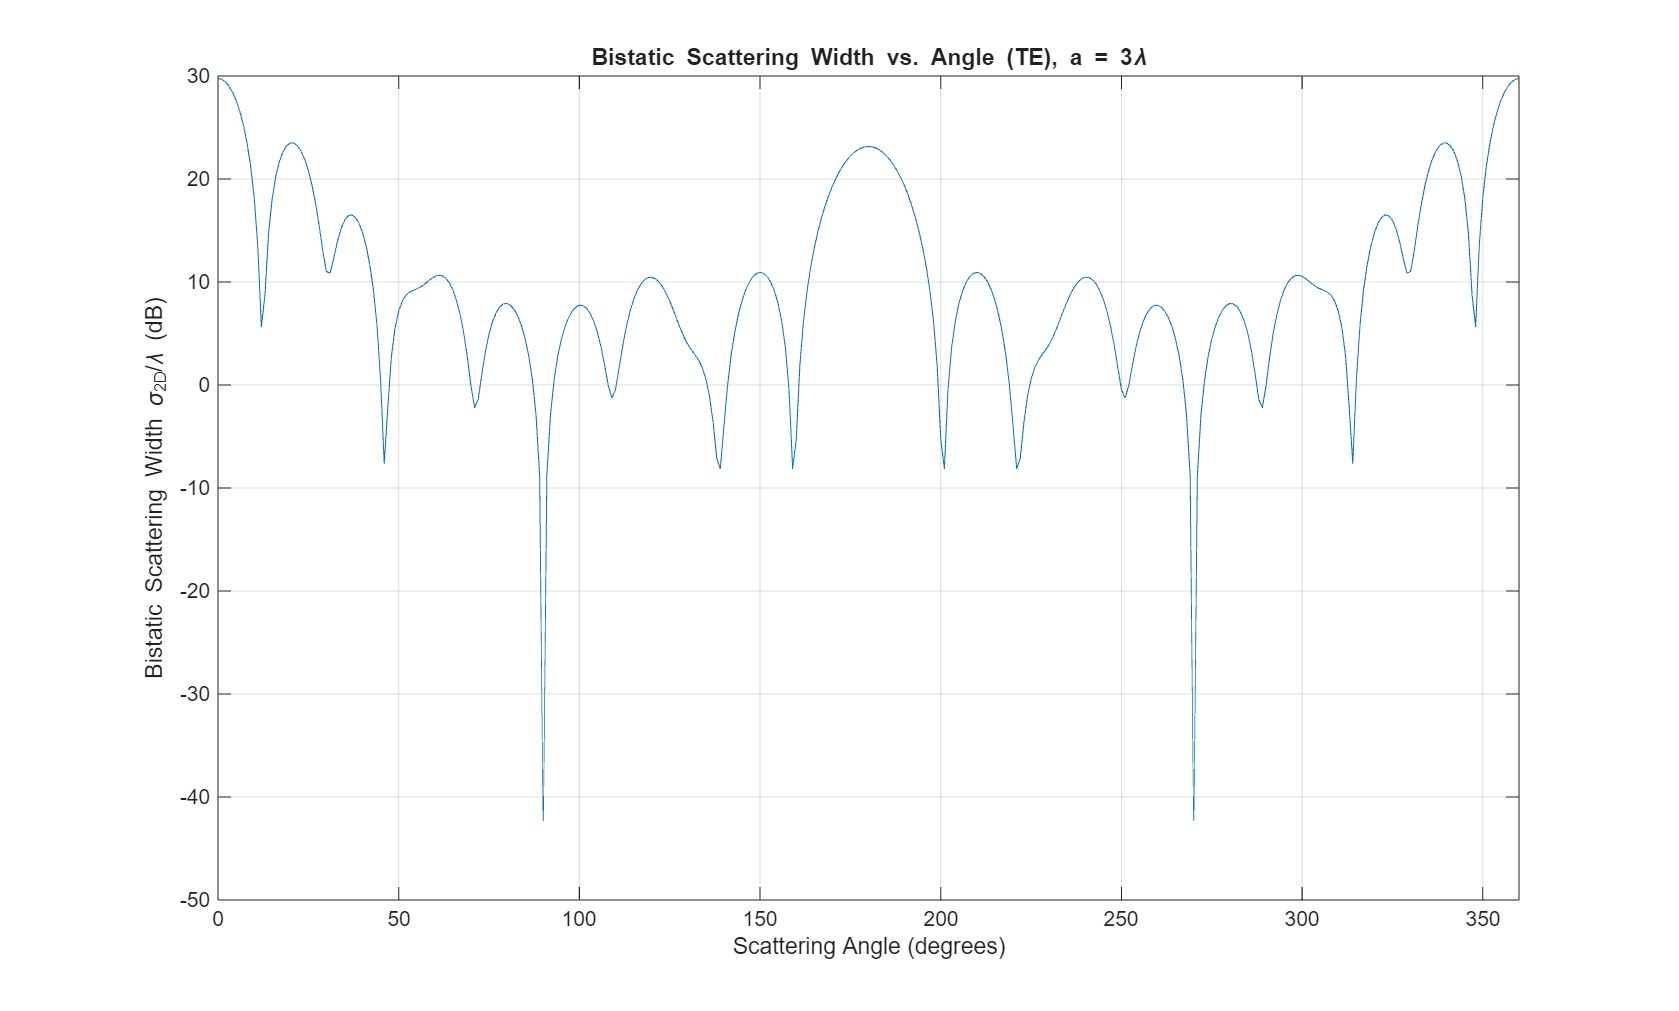
\includegraphics[width=\textwidth]{5d.jpg}
        \caption{TE bistatic scattering width for 3$\lambda$ cylinder.}
    \end{subfigure}
    \caption{Bistatic scattering width for TM and TE polarizations. (a) and (b) show the TM bistatic scattering width for 1$\lambda$ and 3$\lambda$ cylinders, respectively. (c) and (d) show the TE bistatic scattering width for 1$\lambda$ and 3$\lambda$ cylinders, respectively.}
    \label{fig:bistatic_scattering_width}
\end{figure}

The bistatic scattering width for TE polarization exhibits deep valleys at specific angles due to destructive interference between the incident and scattered fields. These valleys correspond to directions where the scattered field cancels out the incident field, resulting in minimal scattered power. This phenomenon is more pronounced for TE polarization because the surface currents generate standing wave patterns that lead to phase cancellations at certain observation angles. In contrast, TM polarization does not exhibit such deep valleys due to the absence of significant standing wave interference effects.

\section{Conclusion}
This paper has presented analysis of electromagnetic scattering from square conducting cylinders using the Method of Moments. We have implemented numerical solutions for both TE and TM polarizations, investigating cylinders with side lengths of 1$\lambda$ and 3$\lambda$. The results demonstrate significant differences between TE and TM polarizations, particularly in the surface current distributions, where TM polarization exhibits sharp peaks at corners while TE polarization shows continuous standing wave patterns. Field distribution analysis reveals increasingly complex interference patterns as the electrical size increases. Additionally, the bistatic scattering width patterns highlight fundamental differences in the scattering mechanisms between the two polarizations.

\begin{thebibliography}{9}
    \bibitem{jin2015theory} J.-M. Jin, \emph{Theory and Computation of Electromagnetic Fields}. Wiley, 2015.
\end{thebibliography}

\end{document}